% Created by tikzDevice version 0.12 on 2019-04-03 19:28:26
% !TEX encoding = UTF-8 Unicode
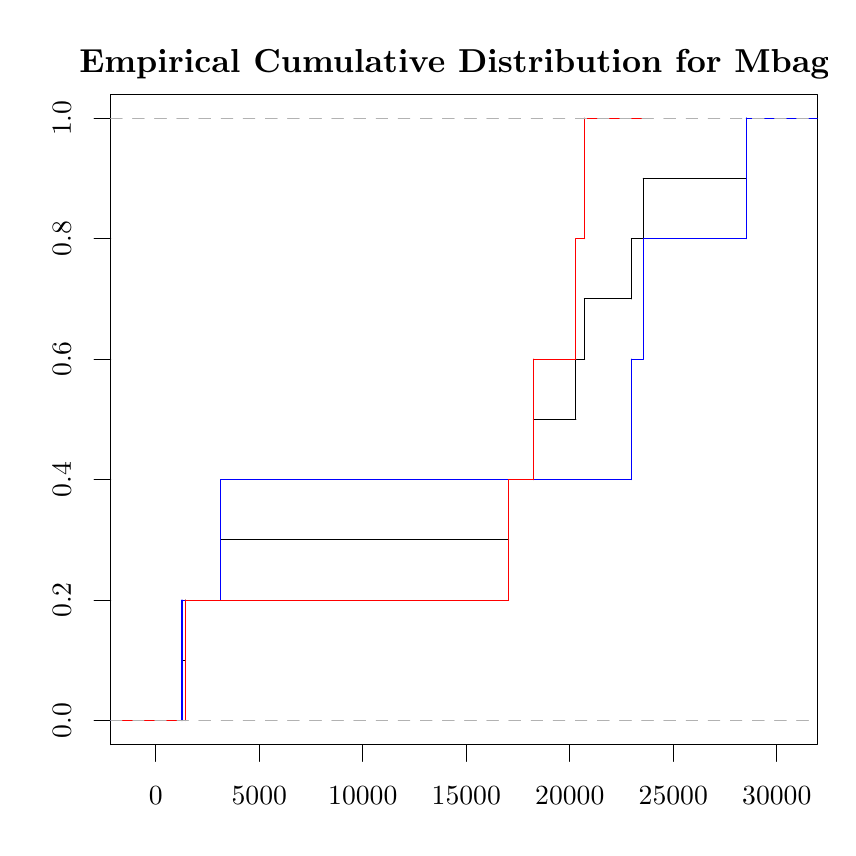
\begin{tikzpicture}[x=1pt,y=1pt]
\definecolor{fillColor}{RGB}{255,255,255}
\path[use as bounding box,fill=fillColor,fill opacity=0.00] (0,0) rectangle (289.08,289.08);
\begin{scope}
\path[clip] (  0.00,  0.00) rectangle (289.08,289.08);
\definecolor{drawColor}{RGB}{0,0,0}

\path[draw=drawColor,line width= 0.4pt,line join=round,line cap=round] ( 46.29, 30.00) -- (270.69, 30.00);

\path[draw=drawColor,line width= 0.4pt,line join=round,line cap=round] ( 46.29, 30.00) -- ( 46.29, 24.00);

\path[draw=drawColor,line width= 0.4pt,line join=round,line cap=round] ( 83.69, 30.00) -- ( 83.69, 24.00);

\path[draw=drawColor,line width= 0.4pt,line join=round,line cap=round] (121.09, 30.00) -- (121.09, 24.00);

\path[draw=drawColor,line width= 0.4pt,line join=round,line cap=round] (158.49, 30.00) -- (158.49, 24.00);

\path[draw=drawColor,line width= 0.4pt,line join=round,line cap=round] (195.89, 30.00) -- (195.89, 24.00);

\path[draw=drawColor,line width= 0.4pt,line join=round,line cap=round] (233.29, 30.00) -- (233.29, 24.00);

\path[draw=drawColor,line width= 0.4pt,line join=round,line cap=round] (270.69, 30.00) -- (270.69, 24.00);

\node[text=drawColor,anchor=base,inner sep=0pt, outer sep=0pt, scale=  1.00] at ( 46.29,  8.40) {0};

\node[text=drawColor,anchor=base,inner sep=0pt, outer sep=0pt, scale=  1.00] at ( 83.69,  8.40) {5000};

\node[text=drawColor,anchor=base,inner sep=0pt, outer sep=0pt, scale=  1.00] at (121.09,  8.40) {10000};

\node[text=drawColor,anchor=base,inner sep=0pt, outer sep=0pt, scale=  1.00] at (158.49,  8.40) {15000};

\node[text=drawColor,anchor=base,inner sep=0pt, outer sep=0pt, scale=  1.00] at (195.89,  8.40) {20000};

\node[text=drawColor,anchor=base,inner sep=0pt, outer sep=0pt, scale=  1.00] at (233.29,  8.40) {25000};

\node[text=drawColor,anchor=base,inner sep=0pt, outer sep=0pt, scale=  1.00] at (270.69,  8.40) {30000};

\path[draw=drawColor,line width= 0.4pt,line join=round,line cap=round] ( 30.00, 38.71) -- ( 30.00,256.37);

\path[draw=drawColor,line width= 0.4pt,line join=round,line cap=round] ( 30.00, 38.71) -- ( 24.00, 38.71);

\path[draw=drawColor,line width= 0.4pt,line join=round,line cap=round] ( 30.00, 82.24) -- ( 24.00, 82.24);

\path[draw=drawColor,line width= 0.4pt,line join=round,line cap=round] ( 30.00,125.77) -- ( 24.00,125.77);

\path[draw=drawColor,line width= 0.4pt,line join=round,line cap=round] ( 30.00,169.31) -- ( 24.00,169.31);

\path[draw=drawColor,line width= 0.4pt,line join=round,line cap=round] ( 30.00,212.84) -- ( 24.00,212.84);

\path[draw=drawColor,line width= 0.4pt,line join=round,line cap=round] ( 30.00,256.37) -- ( 24.00,256.37);

\node[text=drawColor,rotate= 90.00,anchor=base,inner sep=0pt, outer sep=0pt, scale=  1.00] at ( 15.60, 38.71) {0.0};

\node[text=drawColor,rotate= 90.00,anchor=base,inner sep=0pt, outer sep=0pt, scale=  1.00] at ( 15.60, 82.24) {0.2};

\node[text=drawColor,rotate= 90.00,anchor=base,inner sep=0pt, outer sep=0pt, scale=  1.00] at ( 15.60,125.77) {0.4};

\node[text=drawColor,rotate= 90.00,anchor=base,inner sep=0pt, outer sep=0pt, scale=  1.00] at ( 15.60,169.31) {0.6};

\node[text=drawColor,rotate= 90.00,anchor=base,inner sep=0pt, outer sep=0pt, scale=  1.00] at ( 15.60,212.84) {0.8};

\node[text=drawColor,rotate= 90.00,anchor=base,inner sep=0pt, outer sep=0pt, scale=  1.00] at ( 15.60,256.37) {1.0};

\path[draw=drawColor,line width= 0.4pt,line join=round,line cap=round] ( 30.00, 30.00) --
	(285.48, 30.00) --
	(285.48,265.08) --
	( 30.00,265.08) --
	( 30.00, 30.00);
\end{scope}
\begin{scope}
\path[clip] (  0.00,  0.00) rectangle (289.08,289.08);
\definecolor{drawColor}{RGB}{0,0,0}

\node[text=drawColor,anchor=base,inner sep=0pt, outer sep=0pt, scale=  1.20] at (157.74,272.94) {\bfseries Empirical Cumulative Distribution for \textsc{Mbagg}};
\end{scope}
\begin{scope}
\path[clip] ( 30.00, 30.00) rectangle (285.48,265.08);
\definecolor{drawColor}{RGB}{0,0,0}

\path[draw=drawColor,line width= 0.4pt,line join=round,line cap=round] ( 23.15, 38.71) -- ( 55.78, 38.71);

\path[draw=drawColor,line width= 0.4pt,line join=round,line cap=round] ( 55.78, 60.47) -- ( 56.96, 60.47);

\path[draw=drawColor,line width= 0.4pt,line join=round,line cap=round] ( 56.96, 82.24) -- ( 69.73, 82.24);

\path[draw=drawColor,line width= 0.4pt,line join=round,line cap=round] ( 69.73,104.01) -- (173.79,104.01);

\path[draw=drawColor,line width= 0.4pt,line join=round,line cap=round] (173.79,125.77) -- (182.79,125.77);

\path[draw=drawColor,line width= 0.4pt,line join=round,line cap=round] (182.79,147.54) -- (198.09,147.54);

\path[draw=drawColor,line width= 0.4pt,line join=round,line cap=round] (198.09,169.31) -- (201.21,169.31);

\path[draw=drawColor,line width= 0.4pt,line join=round,line cap=round] (201.21,191.07) -- (218.15,191.07);

\path[draw=drawColor,line width= 0.4pt,line join=round,line cap=round] (218.15,212.84) -- (222.45,212.84);

\path[draw=drawColor,line width= 0.4pt,line join=round,line cap=round] (222.45,234.61) -- (259.70,234.61);

\path[draw=drawColor,line width= 0.4pt,line join=round,line cap=round] (259.70,256.37) -- (289.08,256.37);

\path[draw=drawColor,line width= 0.4pt,line join=round,line cap=round] ( 55.78, 38.71) -- ( 55.78, 60.47);

\path[draw=drawColor,line width= 0.4pt,line join=round,line cap=round] ( 56.96, 60.47) -- ( 56.96, 82.24);

\path[draw=drawColor,line width= 0.4pt,line join=round,line cap=round] ( 69.73, 82.24) -- ( 69.73,104.01);

\path[draw=drawColor,line width= 0.4pt,line join=round,line cap=round] (173.79,104.01) -- (173.79,125.77);

\path[draw=drawColor,line width= 0.4pt,line join=round,line cap=round] (182.79,125.77) -- (182.79,147.54);

\path[draw=drawColor,line width= 0.4pt,line join=round,line cap=round] (198.09,147.54) -- (198.09,169.31);

\path[draw=drawColor,line width= 0.4pt,line join=round,line cap=round] (201.21,169.31) -- (201.21,191.07);

\path[draw=drawColor,line width= 0.4pt,line join=round,line cap=round] (218.15,191.07) -- (218.15,212.84);

\path[draw=drawColor,line width= 0.4pt,line join=round,line cap=round] (222.45,212.84) -- (222.45,234.61);

\path[draw=drawColor,line width= 0.4pt,line join=round,line cap=round] (259.70,234.61) -- (259.70,256.37);
\definecolor{drawColor}{gray}{0.70}

\path[draw=drawColor,line width= 0.4pt,dash pattern=on 4pt off 4pt ,line join=round,line cap=round] ( 30.00, 38.71) -- (285.48, 38.71);

\path[draw=drawColor,line width= 0.4pt,dash pattern=on 4pt off 4pt ,line join=round,line cap=round] ( 30.00,256.37) -- (285.48,256.37);
\definecolor{drawColor}{RGB}{0,0,255}

\path[draw=drawColor,line width= 0.4pt,line join=round,line cap=round] (  4.58, 38.71) -- ( 55.78, 38.71);

\path[draw=drawColor,line width= 0.4pt,line join=round,line cap=round] ( 55.78, 82.24) -- ( 69.73, 82.24);

\path[draw=drawColor,line width= 0.4pt,line join=round,line cap=round] ( 69.73,125.77) -- (218.15,125.77);

\path[draw=drawColor,line width= 0.4pt,line join=round,line cap=round] (218.15,169.31) -- (222.45,169.31);

\path[draw=drawColor,line width= 0.4pt,line join=round,line cap=round] (222.45,212.84) -- (259.70,212.84);

\path[draw=drawColor,line width= 0.4pt,line join=round,line cap=round] (259.70,256.37) -- (289.08,256.37);

\path[draw=drawColor,line width= 0.4pt,line join=round,line cap=round] ( 55.78, 38.71) -- ( 55.78, 82.24);

\path[draw=drawColor,line width= 0.4pt,line join=round,line cap=round] ( 69.73, 82.24) -- ( 69.73,125.77);

\path[draw=drawColor,line width= 0.4pt,line join=round,line cap=round] (218.15,125.77) -- (218.15,169.31);

\path[draw=drawColor,line width= 0.4pt,line join=round,line cap=round] (222.45,169.31) -- (222.45,212.84);

\path[draw=drawColor,line width= 0.4pt,line join=round,line cap=round] (259.70,212.84) -- (259.70,256.37);
\definecolor{drawColor}{gray}{0.70}

\path[draw=drawColor,line width= 0.4pt,dash pattern=on 4pt off 4pt ,line join=round,line cap=round] ( 30.00, 38.71) -- (285.48, 38.71);

\path[draw=drawColor,line width= 0.4pt,dash pattern=on 4pt off 4pt ,line join=round,line cap=round] ( 30.00,256.37) -- (285.48,256.37);
\definecolor{drawColor}{RGB}{255,0,0}

\path[draw=drawColor,line width= 0.4pt,line join=round,line cap=round] ( 32.66, 38.71) -- ( 56.96, 38.71);

\path[draw=drawColor,line width= 0.4pt,line join=round,line cap=round] ( 56.96, 82.24) -- (173.79, 82.24);

\path[draw=drawColor,line width= 0.4pt,line join=round,line cap=round] (173.79,125.77) -- (182.79,125.77);

\path[draw=drawColor,line width= 0.4pt,line join=round,line cap=round] (182.79,169.31) -- (198.09,169.31);

\path[draw=drawColor,line width= 0.4pt,line join=round,line cap=round] (198.09,212.84) -- (201.21,212.84);

\path[draw=drawColor,line width= 0.4pt,line join=round,line cap=round] (201.21,256.37) -- (225.51,256.37);

\path[draw=drawColor,line width= 0.4pt,line join=round,line cap=round] ( 56.96, 38.71) -- ( 56.96, 82.24);

\path[draw=drawColor,line width= 0.4pt,line join=round,line cap=round] (173.79, 82.24) -- (173.79,125.77);

\path[draw=drawColor,line width= 0.4pt,line join=round,line cap=round] (182.79,125.77) -- (182.79,169.31);

\path[draw=drawColor,line width= 0.4pt,line join=round,line cap=round] (198.09,169.31) -- (198.09,212.84);

\path[draw=drawColor,line width= 0.4pt,line join=round,line cap=round] (201.21,212.84) -- (201.21,256.37);
\definecolor{drawColor}{gray}{0.70}

\path[draw=drawColor,line width= 0.4pt,dash pattern=on 4pt off 4pt ,line join=round,line cap=round] ( 30.00, 38.71) -- (285.48, 38.71);

\path[draw=drawColor,line width= 0.4pt,dash pattern=on 4pt off 4pt ,line join=round,line cap=round] ( 30.00,256.37) -- (285.48,256.37);
\end{scope}
\begin{scope}
\path[clip] (  0.00,  0.00) rectangle (289.08,289.08);
\definecolor{drawColor}{RGB}{0,0,0}

\node[text=drawColor,rotate= 90.00,anchor=base,inner sep=0pt, outer sep=0pt, scale=  1.00] at ( -2.40,147.54) {Objective function};
\end{scope}
\end{tikzpicture}
